\documentclass[a4paper]{article}
\usepackage{hyperref}
\usepackage{xcolor}
\usepackage{graphicx}
\usepackage[italian]{babel}
\usepackage{cancel}
\usepackage[T1]{fontenc}
\usepackage{url}
\usepackage{import}
\usepackage{nameref}
\usepackage{framed}
\usepackage{multirow}
\usepackage{color}
\usepackage[numbered, framed]{matlab-prettifier}
\usepackage{fancyhdr}
\usepackage{amssymb}
\usepackage{tabu}
\usepackage{mathtools}
\usepackage[margin=2.5cm]{geometry}
\usepackage{listings}
\usepackage{titling}
\usepackage[utf8]{inputenc}


\let\ph\mlplaceholder % shorter macro
\lstMakeShortInline"

\DeclarePairedDelimiter\abs{\lvert}{\rvert}
\newcommand{\bnb}{\begin{nobreak}}
\newcommand{\enb}{\end{nobreak}}

\lstset{
  style              = Matlab-editor,
  basicstyle         = \mlttfamily,
  escapechar         = ",
  mlshowsectionrules = true,
}


\pretitle{%
  \begin{center}
  \LARGE
  
\includegraphics[width=\textwidth/4]{logo_unifi.png}\\[\bigskipamount]
}
\posttitle{\end{center}}
\date{\today}
\input{names.env.tex}

\begin{document}



\title{\vspace{2cm}Elaborato di\\ \textbf{Calcolo Numerico}\\ Anno Accademico 2021/2022\vspace{3cm}}

\author{\wirterOneName{} \emph{\wirterOneSurname{}} - \texttt{\wirterOneId{}} - \textit{\MakeLowercase{\wirterOneName{}}.\MakeLowercase{\wirterOneSurname{}}@stud.unifi.it}
  \and \wirterTwoName{} \emph{\wirterTwoSurname{}} - \texttt{\wirterTwoId{}} - \textit{\MakeLowercase{\wirterTwoName{}}.\MakeLowercase{\wirterTwoSurname{}}@stud.unifi.it}}


\maketitle
\newpage
\tableofcontents
\newpage
\listoffigures
\listoftables


\newpage

\subsection{Esercizio 1} 
Sviluppando  in serie di Taylor in x si ottiene:\\
\[
f(x+h) = f(x) +  hf'(x) + \frac{h^2}{2}f''(x) + \frac{h^3}{6}f'''(x) + O(h^4)
\]
\[
f(x-h) = f(x) -  hf'(x) + \frac{h^2}{2}f''(x) - \frac{h^3}{6}f'''(x) + O(h^4)
\]
Sostituiamo i termini  nell'espressione iniziale:
\[
\frac{ f(x) -  hf'(x) + \frac{h^2}{2}f''(x) - \frac{h^3}{6}f'''(x) + O(h^4) -2f(x) + f(x) +  hf'(x) + \frac{h^2}{2}f''(x) + \frac{h^3}{6}f'''(x) + O(h^4)}{h^2} = \]

\[=\frac{h^2f''(x) + O(h^4)}{h^2} = f''(x) + O(h^2)
\]
\section{\textbf{Capitolo 2}}
\subsection{Esercizio 5}
Scrivere function Matlab distinte che implementino efficientemente i seguenti metodi
per la ricerca degli zeri di una funzione $f(x)$:
\begin{itemize}
    \item il metodo di Newton;
    \item il metodo delle secanti;
    \item il metodo di Steffensen:
\end{itemize}
\begin{eqnarray*}
    x_{n+1}=x_n - \frac{f(x_n)^2}{f(x_n + f(x_n)) - f(x_n)}, & & \mbox{n=0,1,...}
\end{eqnarray*}
Per tutti i metodi, utilizzare come criterio di arresto
\[
    \abs{x_{n+1} - x_n} \leq tol * (1 + \abs{x_n})
\]
essendo $tol$ una opportuna tolleranza specificata in ingresso. Curare particolarmente la robustezza
del codice.
\newline \textbf{Soluzione:} \newline
\begin{itemize}
    \item Metodo di Newton
          \lstinputlisting{capitolo2/es5_newton.m}
    \item Metodo delle secanti
          \lstinputlisting{capitolo2/es5_secanti.m}
    \item Metodo di Steffensen
          \lstinputlisting{capitolo2/es5_steffensen.m}
\end{itemize}

\subsection{Esercizio 6}
Utilizzare le $function$ del precedente esercizio per determinare una approssimazione
della radice della funzione
\[
        f(x) = x - cos(\frac{\pi}{2}x),
\]
per $tol = 10^{-3}, 10^{-6}, 10^{-9}, 10^{-12},$ partendo da $x_0 = 1$
(e $x_1 = 0.99$ per il metodo delle secanti). Tabulare i risultati,
in modo da confrontare le iterazioni richieste da ciascun metodo. Commentare
il relativo costo computazionale, in termini di valutazioni funzionali richieste.
\newline \textbf{Soluzione:}








Eseguendo lo script \nameref{cod:6}si ottengono i risultati contenuti nella tabella \ref{tab:6}
e nella figura \ref{fig:es6}. Come si può notare, il metodo di newton e il metodo delle secanti
convergono molto più rapidamente del metodo di bisezione e del metodo delle corde.
\begin{table}[h]
        \renewcommand\arraystretch{2}
        \begin{tabular}{|l l l l l|}
                \hline
                Metodo     & tolleranza$=10^{-3}$ & tolleranza$=10^{-6}$ & tolleranza$=10^{-9}$ & tolleranza$=10^{-12}$ \\
                \hline
                newton     & 5.94611646360541e-01 & 5.94611644056836e-01 & 5.94611644056836e-01 & 5.94611644056836e-01  \\
                secanti    & 5.94611646954077e-01 & 5.94611644056836e-01 & 5.94611644056836e-01 & 5.94611644056836e-01  \\
                steffensen & 5.94611681141925e-01 & 5.94611644056837e-01 & 5.94611644056836e-01 & 5.94611644056836e-01  \\
                \hline
        \end{tabular}
        \caption{valori approssimati con i metodi di Newton, secanti e Steffensen}
        \label{tab:6}
\end{table}
% \newpage
\begin{figure}[h!]
        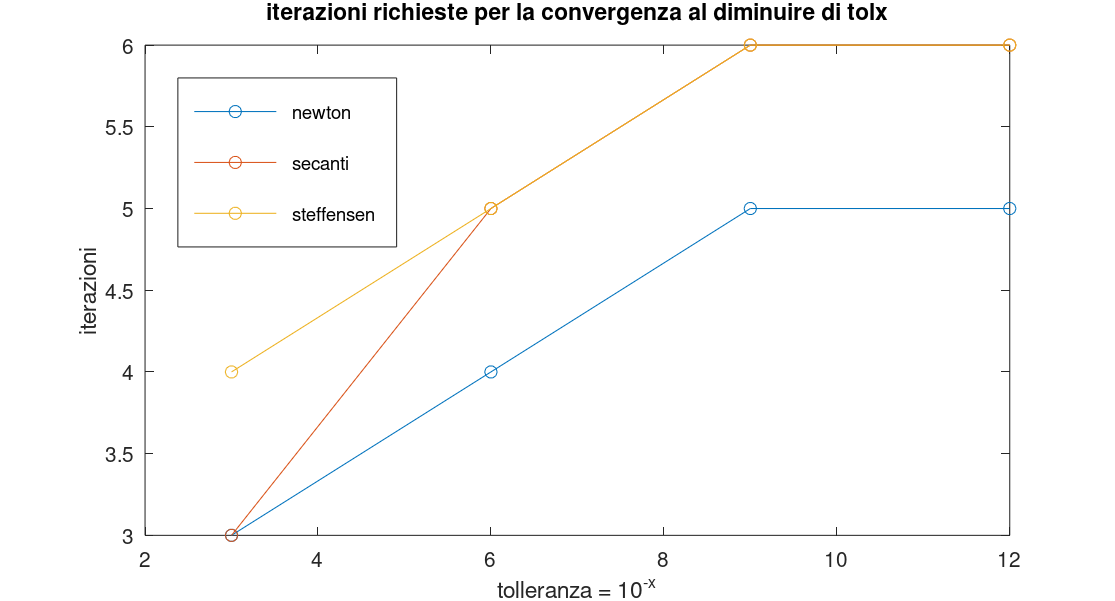
\includegraphics[scale=0.7]{capitolo2/es6_figure.png}
        \caption{iterazioni richieste}
        \label{fig:es6}
\end{figure}




\subsection{Esercizio 7}
Utilizzare le $function$ del precedente esercizio per determinare una approssimazione
della radice della funzione
\[
        f(x) = \left[x - cos(\frac{\pi}{2}x)\right]^3,
\]
per $tol = 10^{-3}, 10^{-6}, 10^{-9}, 10^{-12},$ partendo da $x_0 = 1$
(e $x_1 = 0.99$ per il metodo delle secanti). Tabulare i risultati,
in modo da confrontare le iterazioni richieste da ciascun metodo. Commentare
i risultati ottenuti.
\newline \textbf{Soluzione:}

Eseguendo lo script \nameref{cod:7} si ottengono i risultati contenuti nella tabella \ref{tab:7}
e nella figura \ref{fig:es7}. Come si può notare, il metodo di newton e il metodo delle secanti
convergono molto più rapidamente del metodo di bisezione e del metodo delle corde.
\begin{table}[ht]
        \centering
        \renewcommand\arraystretch{2}
        \resizebox{\columnwidth}{!}{
                \begin{tabular}{|l l l l l|}
                        \hline
                        Metodo                &        & newton                & secanti               & steffensen            \\
                        \hline
                        tolleranza$=10^{-3}$  & \vline & 5.969479343078770e-01 & 5.991437227787725e-01 & 5.973965526716639e-01 \\
                        tolleranza$=10^{-6}$  & \vline & 5.946140179818806e-01 & 5.946156634766230e-01 & 5.946143706333854e-01 \\
                        tolleranza$=10^{-9}$  & \vline & 5.946116464662755e-01 & 5.946116487688006e-01 & 5.946130329177074e-01 \\
                        tolleranza$=10^{-12}$ & \vline & 5.946116440592810e-01 & 5.946116440610053e-01 & 5.946130329177074e-01 \\
                        \hline
                \end{tabular}
        }
        \caption{Valori approssimati per $x - cos^{3}$ con i metodi di Newton, secanti e Steffensen}
        \label{tab:7}
\end{table}
\begin{figure}[!ht]
        \centering
        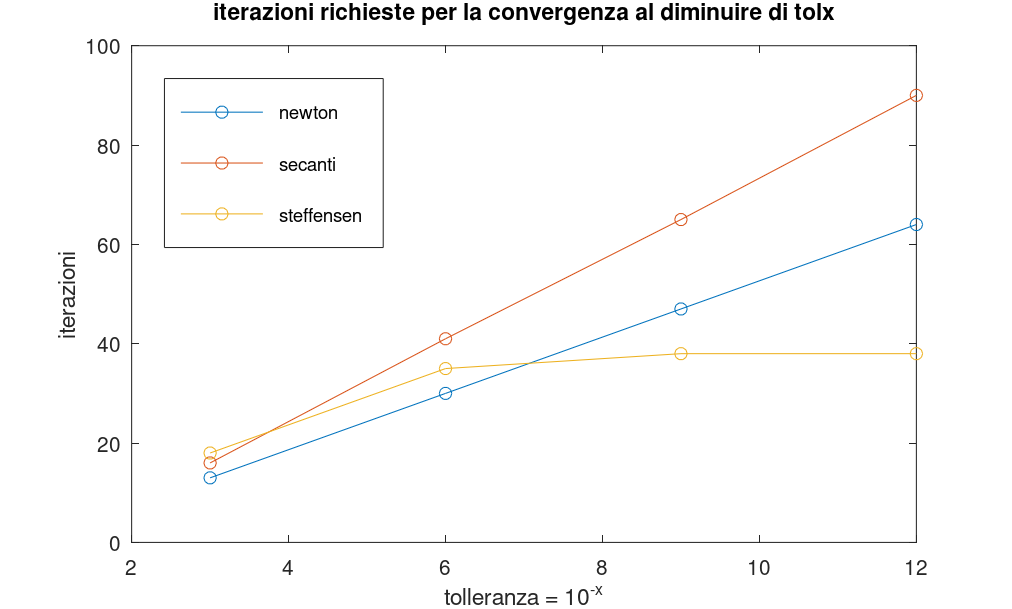
\includegraphics[width=16cm,height=12cm,keepaspectratio]{capitolo2/es7_figure.png}
        \caption{Valori approssimati per $x - cos^{3}$ con i metodi di Newton, secanti e Steffensen}
        \label{fig:es7}
\end{figure}
\FloatBarrier
In iterazione $38$ la funzione con metodo di Steffensen falliscie con valori di tolleranza
$10^-9$ e $10^-12$. Ed infatti, si vede che in questi valori la figura \ref{fig:es7}
rimane costante rispetto iterazioni. Questo fallimento dato da divizione a zero.
\newline \textbf{Costo computazionale} \newline
È possibile valutare i costi computazionali dei algoritmi verificando il numero
di funzioni richiamate all'interno dei codici, mediante feval:
\begin{itemize}
        \item Newton: $2i$, $i=1:maxit$;
        \item Secanti: $1 + i$, $i=1:maxit$;
        \item Steffensen: $2i$, $i=1:maxit$;
\end{itemize}


\section{\textbf{Capitolo 3}}
\subsection{Esercizio 8}
Scrivere una function Matlab,
\begin{lstlisting}[language=Matlab]
    function x = mialu(A, b)
\end{lstlisting}
che, data in ingresso una matrice $A$ ed un vettore $b$, calcoli la soluzione
del sistema lineare $Ax = b$ con il metodo di fattorizzazione $LU$ con pivoting parziale.
Curare particolarmente la scrittura e l'efficienza della function,
e validarla su due esempi non banali, generati casualmente,
di cui sia nota la soluzione.
\newline \textbf{Soluzione:}
\lstinputlisting[language=Matlab]{capitolo3/es8_lu.m}
\subsection{Esercizio 9}
Scrivere una function Matlab,
\begin{lstlisting}
function x = mialdl(A, b)
\end{lstlisting}
che, dati in ingresso una matrice sdp $A$ ed un vettore $b$, calcoli la soluzione
del corrispondente sistema lineare utilizzando la fattorizzazione $LDL^T$.
Curare particolarmente la scrittura e l'efficienza della function,
e validarla su due esempi non banali, generati casualmente, di cui sia nota la soluzione.
\newline \textbf{Soluzione:}

\lstinputlisting{matlab/capitolo3/mialdl.m}
Eseguendo lo script \nameref{cod:9} si ottengono i risultati contenuti nelle
tabelle \ref{tab:9_1} e \ref{tab:9_2}.

Prima sistema lineare è
\[
   \begin{bmatrix}
      166 & 105 & 161 & 132 \\
      105 & 119 & 151 & 98  \\
      161 & 151 & 239 & 144 \\
      132 & 98  & 144 & 131
   \end{bmatrix}
   \begin{bmatrix}
      x_{1} \\
      x_{2} \\
      x_{3} \\
      x_{4}
   \end{bmatrix}
   =
   \begin{bmatrix}
      5  \\
      10 \\
      6  \\
      2
   \end{bmatrix}
\]
Invece seconda sistema lineare è
\[
   \begin{bmatrix}
      45 & 27 \\
      27 & 18
   \end{bmatrix}
   \begin{bmatrix}
      x_{1} \\
      x_{2}
   \end{bmatrix}
   =
   \begin{bmatrix}
      2 \\
      5
   \end{bmatrix}
\]
Eseguendo la funzione creata \lstinline{mialdl} e comando interno di
matlab \lstinline{A\b}, possiamo confrontare il risultati di funzione
scritta con quello realizzato nativamente in matlab.
\begin{table}[ht]
   \centering
   \renewcommand\arraystretch{2}
   \begin{tabular}{|l | c c |}
      \hline
      $x$     & $mialdl$               & $A \backslash b$       \\
      \hline
      $x_{1}$ & 9.752409097697867e-02  & 9.752409097697871e-02  \\
      $x_{2}$ & 2.974225536634357e-01  & 2.974225536634358e-01  \\
      $x_{3}$ & -1.315833858151011e-01 & -1.315833858151011e-01 \\
      $x_{4}$ & -1.608594100046056e-01 & -1.608594100046056e-01 \\
      \hline
   \end{tabular}
   \caption{Confronto di soluzioni di \lstinline{mialdl} e $A \backslash b$ per primo sistema}
   \label{tab:9_1}
\end{table}
\begin{table}[ht]
   \centering
   \renewcommand\arraystretch{2}
   \begin{tabular}{| l | c c |}
      \hline
      $x$     & $mialdl$               & $A \backslash b$       \\
      \hline
      $x_{1}$ & -1.222222222222222e+00 & -1.222222222222221e+00 \\
      $x_{2}$ & 2.111111111111110e+00  & 2.111111111111110e+00  \\
      \hline
   \end{tabular}
   \caption{Confronto di soluzioni di \lstinline{mialdl} e $A \backslash b$ per secondo sistema}
   \label{tab:9_2}
\end{table}
\FloatBarrier

\subsection{Esercizio 10}
Data la function Matlab
\lstinputlisting{capitolo3/es10_linsis.m}
che crea sistemi lineari casuali con soluzione nota, risolvere, utilizzando la \textit{function} \lstinline{mialu}, i sistemi
lineari generati da \lstinline{[A,b]=linsis(10,1)} e \lstinline{[A,b]=linsis(10,10)}. Commentare l'accuratezza dei
risultati ottenuti, dandone spiegazione esaustiva.
\newline \textbf{Soluzione:} \newline
\begin{lstlisting}
>> [A, b] = linsis(10, 1); es8_lu(A,b)
ans =

    1
    2
    3
    4
    5
    6
    7
    8
    9
   10

>> [A, b] = linsis(10, 10); es8_lu(A,b)
ans =

  -307.6448
   386.6526
   184.3573
  -342.4373
   185.5085
   551.9206
  -137.7750
    70.6324
    -4.2105
  -608.0000

>>
\end{lstlisting}
Nel \textbf{primo caso} notiamo che l'errore é uguale a zero, infatti abbiamo che i soluzioni di $A$
sono tutti come aspettati: \lstinline{ans = [1; 2; 3; 4; 5; 6; 7; 8; 9; 10]}
\newline
Considerando che la soluzione con perturbazioni consiste nel risolvere il sistema
lineare $A(\epsilon)x(\epsilon) = b(\epsilon)$, dato che $\epsilon = 0 \rightarrow x(0) = x$
la soluzione senza perturbazione.
\newline
\newline
Nel \textbf{secondo caso} calcolando il numero di condizionamento
$K(A^T\cdot A) = \|A^T A\|\cdot\|(A^T A)^{-1}\|$ abbiamo che $K = 10^{16}$
Avendo $k \gg 1$ si ha un mal condizionamento del problema.

\subsection{Esercizio 11}
Scrivere una function Matlab,
\begin{lstlisting}[language=Matlab]
    function [x,nr] = miaqr(A, b)
\end{lstlisting}
che, data in ingresso la matrice $A$ $m \times n$, con $m \geq n = rank(A)$, ed un vettore $b$ di lunghezza
$m$, calcoli la soluzione del sistema lineare $Ax = b$ nel senso dei minimi quadrati e, inoltre, la
norma, $nr$, del corrispondente vettore residuo. Curare particolarmente la scrittura e l'efficienza della
\textit{function}. Validare la \textit{function} $miaqr$ su due esempi non banali, generati casualmente, confrontando
la soluzione ottenuta con quella calcolata con l'operatore Matlab.
\newline \textbf{Soluzione:}
\lstinputlisting[language=Matlab]{capitolo3/es11_qr.m}
\subsection{Esercizio 12}
Scrivere una function Matlab,
\begin{lstlisting}
function [x,nr] = miaqr(A, b)
\end{lstlisting}
che, data in ingresso la matrice $A$ $m \times n$, con $m \geq n = rank(A)$, ed un vettore $b$ di lunghezza
$m$, calcoli la soluzione del sistema lineare $Ax = b$ nel senso dei minimi quadrati e, inoltre, la
norma, $nr$, del corrispondente vettore residuo. Curare particolarmente la scrittura e l'efficienza della
\textit{function}. Validare la \textit{function} \lstinline{miaqr} su due esempi non banali,
generati casualmente, confrontando la soluzione ottenuta con quella calcolata con l'operatore Matlab.
\newline \textbf{Soluzione:}

\lstinputlisting{matlab/capitolo3/miaqr.m}
Eseguendo lo script \nameref{cod:12} si ottengono i risultati contenuti nelle
tabelle \ref{tab:12_1} e \ref{tab:12_2}.

Prima sistema lineare è
\[
   \begin{bmatrix}
      3  & 9 & 8 & 9 \\
      4  & 1 & 9 & 1 \\
      10 & 2 & 6 & 1 \\
      9  & 3 & 8 & 9
   \end{bmatrix}
   \begin{bmatrix}
      x_{1} \\
      x_{2} \\
      x_{3} \\
      x_{4}
   \end{bmatrix}
   =
   \begin{bmatrix}
      3 \\
      1 \\
      1 \\
      9
   \end{bmatrix}
\]
Invece seconda sistema lineare è
\[
   \begin{bmatrix}
      6  & 6 \\
      10 & 7 \\
      6  & 9
   \end{bmatrix}
   \begin{bmatrix}
      x_{1} \\
      x_{2}
   \end{bmatrix}
   =
   \begin{bmatrix}
      10 \\
      8  \\
      10
   \end{bmatrix}
\]
Eseguendo la funzione creata \lstinline{miaqr} e comando interno di
matlab \lstinline{r\c}, possiamo confrontare il risultati di funzione
scritta con quello realizzato nativamente in matlab.
\begin{table}[ht]
   \centering
   \renewcommand\arraystretch{2}
   \begin{tabular}{|l | c c |}
      \hline
      $x$     & $miaqr$                & $r \backslash c$       \\
      \hline
      $x_{1}$ & 1.491803278688525e-01  & 1.491803278688524e-01  \\
      $x_{2}$ & -8.508196721311473e-01 & -8.508196721311487e-01 \\
      $x_{3}$ & 1.475409836065585e-02  & 1.475409836065600e-02  \\
      $x_{4}$ & 1.121311475409836e+00  & 1.121311475409836e+00  \\
      \hline
   \end{tabular}
   \caption{Confronto di soluzioni di \lstinline{miaqr} e $r \backslash c$ per primo sistema}
   \label{tab:12_1}
\end{table}
\FloatBarrier
\begin{table}[ht]
   \centering
   \renewcommand\arraystretch{2}
   \begin{tabular}{| l | c c |}
      \hline
      $x$     & $miaqr$               & $r \backslash c$      \\
      \hline
      $x_{1}$ & 8.130081300812995e-02 & 8.130081300813012e-02 \\
      $x_{2}$ & 1.162601626016260e+00 & 1.162601626016260e+00 \\
      \hline
   \end{tabular}
   \caption{Confronto di soluzioni di \lstinline{miaqr} e $r \backslash c$ per secondo sistema}
   \label{tab:12_2}
\end{table}
Per dimostrare che risultato è corretto stato utilizzato il metodo discritto sul
\href{https://it.mathworks.com/help/matlab/ref/qr.html}{pagina di descrizione di funzione qr}
\FloatBarrier

\subsection{Esercizio 13}
Utilizzare la \textit{function} $miaqr$ per risolvere, nel senso dei minimi quadrati,
i sistemi lineari sovradeterminati
\begin{eqnarray*}
    \mbox{A x = b,} & & \mbox{(D*A)x = (D*b)}
\end{eqnarray*}
definiti dai seguenti dati:
\begin{lstlisting}
A = [ 1 3 2; 3 5 4; 5 7 6; 3 6 4; 1 4 2 ];
b = [ 15 28 41 33 22 ]';
D = diag(1:5);
\end{lstlisting}
Commentare i risultati ottenuti.
\newline \textbf{Soluzione:}

\lstinputlisting{./capitolo3/es13.m}
Il risultato finale è $ ris =\left(\begin{array}{c}
    1 \\
    2 \\
    3 \\
\end{array}\right)$  

\subsection{Esercizio 14}

\begin{table}[h]
\begin{tabular}{|l l|}
        \hline
        A$\backslash$b & (A’*A)$\backslash$(A’*b)\\
        \hline
        1.0000& 3.5759 \\
    	2.0000&-3.4624   \\
    	3.0000&  9.5151\\
    	4.0000&-1.2974\\
    	5.0000& 7.9574\\
    	6.0000& 4.9125\\
    	7.0000& 7.2378\\
    	8.0000& 7.9765\\
        \hline
\end{tabular}
\caption{valori approssimati}
\label{tab:14}     
\end{table}

L'espressione $A \backslash b$ risolve in matlab,  il sistema di equazioni lineari nella forma matriciale $A\cdot x=b$ per x.
L'espressione $(A^{T}\cdot A) \backslash (A^{T} \cdot b)$, è matematicamente la stessa operazione dell'espressione precedente, solamente che si moltiplica le due componenti per la trasposta di A. 
La matrice A viene calcolata usando la funzione vander() che genera una matrice di tipo Vandermonde, la quale è  mal condizionata. Usando la funzione cond() sulla matrice A si ottiene una condizionamento pari a: 1.5428e+09.Nella prima espressione, questo malcondizionamento non influisce sul risultato.Invece nella seconda espressione eseguendo la prima parentesi tonda, il condizionamento è pari a: 4.4897e+18. Questo fa si che eseguendo la divisione tra una matrice mal condizionata e il vettore, il risultato presenta degli errori.
\section{Capitolo 4}
\subsection{Esercizio 15}
Usare la \textit{function} del precedente esercizio per risolvere, a partire dal vettore iniziale
nullo, i seguenti sistemi nonlineari, utilizzando tolleranze $tol = 1e-3$, $1e-8$, $1e-13$:
\begin{eqnarray*}
    f_1(x) = \left(\begin{array}{c}
        (x^{2}_{1} + 1)(x_2 - 2) \\
        exp(x_1 - 1) + exp(x_2 - 2) - 2
    \end{array}\right), & & f_2(x) = \left(\begin{array}{c}
        x_1 - x_2x_3                   \\
        exp(x_1 + x_2 + x_3 - 3) - x_2 \\
        x_1 + x_2 + 2x_3 - 4
    \end{array}\right).
\end{eqnarray*}
Tabulare i risultati ottenuti, commentandone l'accuratezza.
\newline \textbf{Soluzione:}

Eseguendo lo script \nameref{cod:15} si ottengono i risultati contenuti nella tabella \ref{tab:15}
e nella figura \ref{fig:es15}.
\begin{table}[h]
    \renewcommand\arraystretch{2}
    \resizebox{\columnwidth}{!}{
        \begin{tabular}{|l l l l l|}
            \hline
            Funzione   & \vline & tolleranza$=10^{-3}$  & tolleranza$=10^{-8}$  & tolleranza$=10^{-13}$ \\
            \hline
            $f_1(x_1)$ & \vline & 1.000119399056337e+00 & 1.000000007127784e+00 & 1.000000000000000e+00 \\
            $f_1(x_2)$ & \vline & 2.000000000000000e+00 & 2.000000000000000e+00 & 2.000000000000000e+00 \\
            \hline
            $f_2(x_1)$ & \vline & 9.999998150012226e-01 & 1.000000000000042e+00 & 1.000000000000042e+00 \\
            $f_2(x_2)$ & \vline & 9.999997068384456e-01 & 9.999999999999842e-01 & 9.999999999999842e-01 \\
            $f_2(x_3)$ & \vline & 1.000000239080166e+00 & 9.999999999999871e-01 & 9.999999999999871e-01 \\
            \hline
        \end{tabular}
    }
    \caption{valori approssimati con i metodi di Newton, secanti e Steffensen}
    \label{tab:15}
\end{table}
\begin{figure}[!ht]
    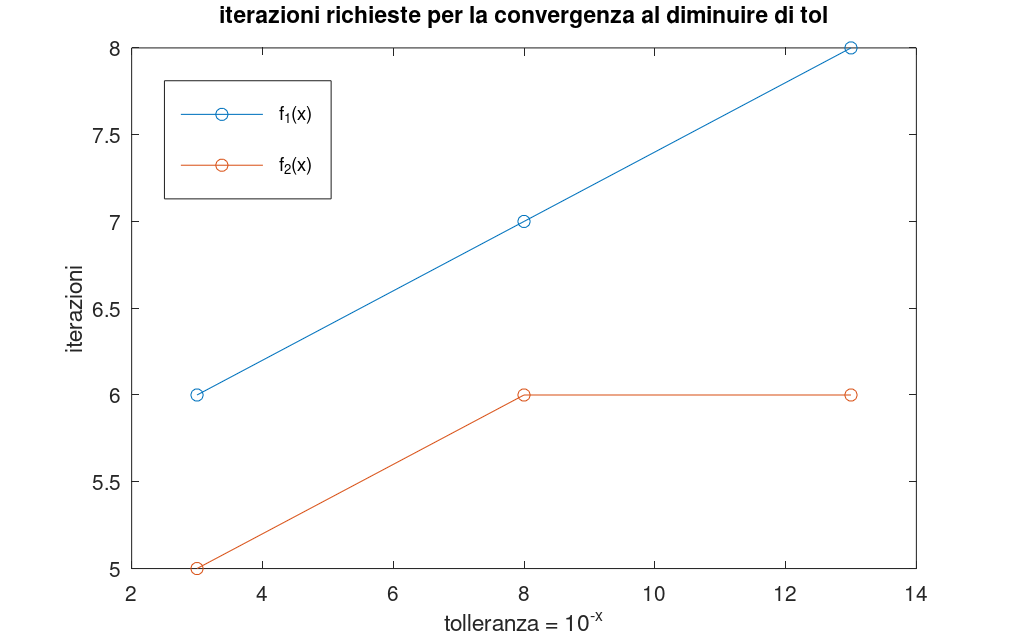
\includegraphics[width=16cm,height=12cm,keepaspectratio]{capitolo4/es15_figure.png}
    \caption{iterazioni richieste}
    \label{fig:es15}
\end{figure}
\newline
Come si vede da risultati ottentui l'accuratezza di funzione di esercizio precedente
rispetta la tolleranza richiesta, quindi criterio di arresto è stato scielto in modo giusto.

Parlando di iterazioni richeiste, si vede, che in funzione con più esponenziali, cioè prima
sono richiesti più iterazioni dato la più alta complessità dei calcoli.

\subsection{Esercizio 16}
Eseguendo \nameref{cod:16} si ottiene:\\
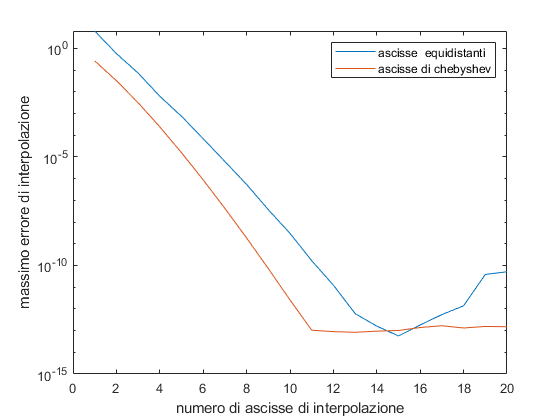
\includegraphics[scale=0.8]{capitolo4/hermite.png}
\section{Capitolo 5}
\subsection{Esercizio 21}
\lstinputlisting[language=Matlab]{./capitolo5/ncweights.m}
Eseguendo lo script \ref{cod:21} si ottiene:
\begin{table}[h]
    \centering
    \renewcommand\arraystretch{3}
    \begin{tabular}{|l|c|c|c|c|c|c|c|c|}
        \hline
        n $\backslash c_{in}$ & 0 & 1 & 2 & 3 & 4 & 5 & 6 & 7 \\
        \hline
        1 & $\dfrac{1}{2}$ & $\dfrac{1}{2}$ & & & & &  &\\
        \hline
        2 & $\dfrac{1}{3}$ & $\dfrac{4}{3}$ & $\dfrac{1}{3}$ & & & &&\\
        \hline
        3 &  $\dfrac{3}{8}$ & $\dfrac{9}{8}$ & $\dfrac{9}{8}$ & $\dfrac{3}{8}$ & & & & \\
        \hline
        4 & $\dfrac{14}{45} $ & $\dfrac{64}{45} $ & $\dfrac{8}{15} $ & $\dfrac{64}{45} $ &$\dfrac{14}{45} $ &&&\\
        \hline
        5 & $\dfrac{95}{288}$ & $\dfrac{95}{288}$ & $\dfrac{95}{288}$ & $\dfrac{95}{288}$ & $\dfrac{95}{288}$ & $\dfrac{95}{288}$ &&\\
        \hline
        6 & $\dfrac{41}{140}$ & $\dfrac{54}{35}$ & $\dfrac{27}{140}$ & $\dfrac{68}{35}$ & $\dfrac{27}{140}$ & $\dfrac{54}{35}$ & $\dfrac{41}{140}$ &\\
        \hline
        7 & $\dfrac{108}{355}$ & $\dfrac{810}{559}$ & $\dfrac{343}{640}$ & $\dfrac{649}{536}$ & $\dfrac{649}{536}$  & $\dfrac{343}{640}$ & $\dfrac{810}{559}$ & $\dfrac{108}{355}$\\
        \hline
    \end{tabular}
    \caption{pesi della formula di Newton-Cotes fino al settimo grado}
\end{table}
\subsection{Esercizio 22}
Tabulare il massimo errore di approssimazione (stimato su 10001 punti equidistanti
in $[0, 1]$) ottenuto approssimando le funzioni
\[
    \begin{array}{ccccc}
        sin(2\pi x) & & e & & cos(2\pi x)
    \end{array}
\]
mediante le function $spline0$ e $spline$, interpolanti su $n + 1$ punti equidistanti in $[0, 1]$,
per $n = 5, 10, 15, 20, \dots, 50$. Commentare i risultati ottenuti.
\newline \textbf{Soluzione:}

Eseguendo lo script \nameref{cod:22} si ottengono i risultati contenuti nella tabella \ref{tab:22}
e nella figura \ref{fig:es22}, che rappresenta il logaritmo di errore di interpolazione data
eccessiva differenza tra alcuni valori.
\begin{table}[h]
    \renewcommand\arraystretch{2}
    \resizebox{\columnwidth}{!}{
        \begin{tabular}{| l l l l l l|}
            \hline
            Numero di punti & \vline & spline0 sin           & spline sin            & spline0 cos           & spline cos            \\
            \hline
            5               & \vline & 2.001701314863913e-02 & 1.807582872673141e-01 & 1.610187576696707e-01 & 2.001701314863924e-02 \\
            10              & \vline & 6.866934777143285e-04 & 4.406993304975182e-03 & 2.548906760377223e-02 & 4.997949001644519e-03 \\
            15              & \vline & 1.110611957051422e-04 & 5.108853724136997e-04 & 1.015096384509251e-02 & 1.022458829215145e-03 \\
            20              & \vline & 3.189430039152175e-05 & 1.128798996133107e-04 & 5.445736215755059e-03 & 3.179572242010265e-04 \\
            25              & \vline & 1.233796729405157e-05 & 3.536684739838258e-05 & 3.394941446614230e-03 & 1.278076383067761e-04 \\
            30              & \vline & 5.797512077632128e-06 & 1.378425643952519e-05 & 2.318648806181711e-03 & 6.067991993707889e-05 \\
            35              & \vline & 3.063198617536678e-06 & 6.237243845463869e-06 & 1.684034317896432e-03 & 3.234496704618284e-05 \\
            40              & \vline & 1.764375267554463e-06 & 3.145724463402000e-06 & 1.278527355775938e-03 & 1.876829765667942e-05 \\
            45              & \vline & 1.085622804652964e-06 & 1.722751742837259e-06 & 1.003721436690030e-03 & 1.162001372967403e-05 \\
            50              & \vline & 7.065852024590313e-07 & 1.006498800408540e-06 & 8.089237478392519e-04 & 7.571318735410948e-06 \\
            \hline
        \end{tabular}
    }
    \caption{valori approssimati con i metodi spline0 e spline}
    \label{tab:22}
\end{table}
\begin{figure}[!ht]
    \centering
    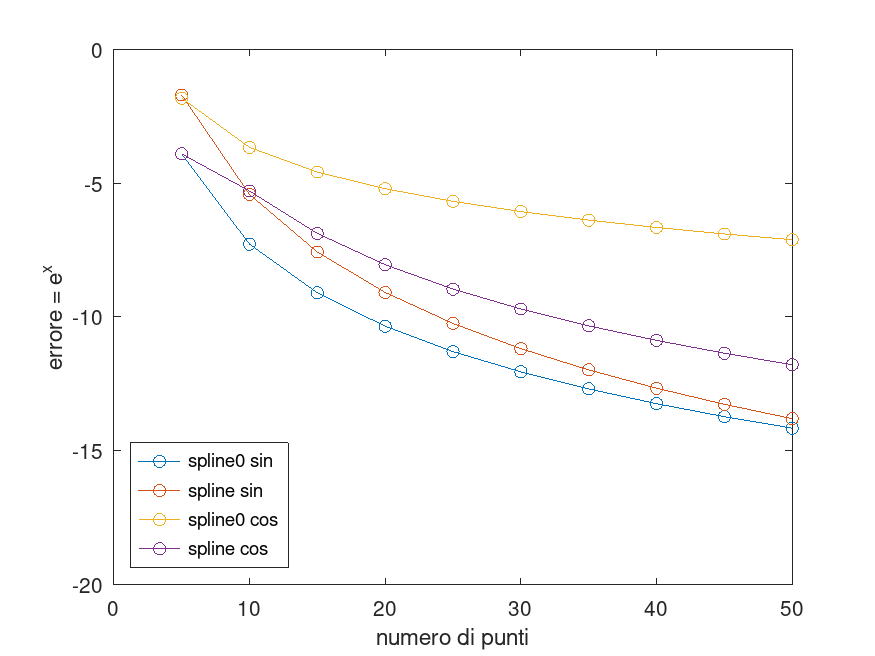
\includegraphics[width=16cm,height=12cm,keepaspectratio]{capitolo5/es22_figure.png}
    \caption{logaritmo di errore}
    \label{fig:es22}
\end{figure}
In base ai risultati ottenuti, si constata che la spline knot-a-not implementata da
Matlab restituisce degli errori di approssimazione significativamente più bassi
per quanto riguarda la funzione $f(x) = cos(2 \pi x)$. Si osserva invece che i risultati
ottenuti per $f(x) = sin(2 \pi x)$ si discostano meno tra di loro. Il motivo di ciò è
che le spline cubiche naturali hanno un piccolo errore agli estremi dovuto alle
condizioni iniziali imposte. Ovvero, data $f(x) = cos(2 \pi x)$:
\[
    f'(0) = f''(1) = -4 \pi ^2
\]
Osserviamo che questo errore non si presenta con $f(x) = sin(2 \pi x)$. Infatti:
\[
    f''(0) = f''(1) = 0
\]

% \newpage
\subsection{Esercizio 23}
Sia assegnata la seguente perturbazione della funzione $f(x) = sin(\pi x^2)$:
\[
    \tilde{f}(x) = f(x) + 10^{-1} rand(size(x)),
\]
in cui $rand$ è la function built-in di Matlab. Calcolare polinomio di approssimazione ai minimi
quadrati di grado $m$, $p(x)$, sui dati $(x_i, \tilde{f}(x_i))$, $i = 0, \dots, n$, con:
\begin{eqnarray*}
    x_i = i/n, & & n = 10^4.
\end{eqnarray*}
Graficare (in formato $semilogy$) l'errore di approssimazione $\|f - p\|$ (stimato come il massimo
errore sui punti $x_i$), relativo all'intervallo $[0, 1]$, rispetto ad $m$, per $m = 1, 2, \dots, 15$.
Commentare i risultati ottenuti.
\newline \textbf{Soluzione:}

Eseguendo lo script \nameref{cod:23} si ottengono i risultati contenuti nella figura \ref{fig:es22}.
\begin{figure}[!ht]
    \centering
    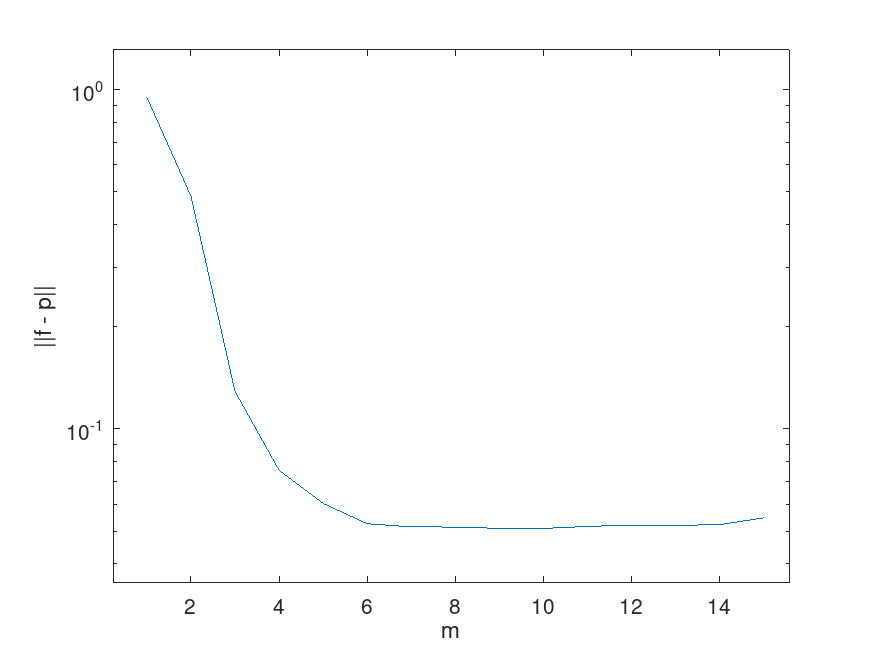
\includegraphics[width=16cm,height=10cm,keepaspectratio]{capitolo5/es23_figure.png}
    \caption{logaritmo di errore}
    \label{fig:es23}
\end{figure}
\FloatBarrier
L'errore decresce molto velocemente inizialmente, ma superato il valore di $m = 5$, si stabilizza
senza azzerarsi.

\subsection{Esercizio 24}
Costruire una function Matlab che, dato in input $n$, restituisca i pesi della quadratura
della formula di Newton-Cotes di grado $n$. Tabulare, quindi, i pesi delle formule di grado
1, 2, \dots, 7 e 9 (come numeri razionali).
\newline \textbf{Soluzione:} \newline
% \lstinputlisting{capitolo5/trapecomp.m}
% \lstinputlisting{capitolo5/simpcomp.m}
% Approssimando $\displaystyle \int_{-1}^{1.1}tan(x)dx$ con le due formule si ottiene:
% \begin{table}[h]
%     \begin{tabular}{|c|c|c |}
%     \hline
%     intervalli$\backslash$formula & trapezi composita         &simpson composita\\
%     \hline
%     $2$                           &$0.266403558406035$        &$0.266403558406035$ \\
%     $4$                           &$0.203432804450016$        &$0.182442553131343$ \\
%     $6$                           &$0.188498346613972$        &$0.177333443886033$ \\
%     $8$                           &$0.182789408875225$        &$0.175908277016961$ \\
%     $10$                          &$0.180034803521960$        &$0.175392868382289$ \\
%     $12$                          &$0.178504015707472$        &$0.175172572071972$ \\
%     $14$                          &$0.177568218195411$        &$0.175066546519247$ \\
%     $16$                          &$0.176955413111201$        &$0.175010747856527$ \\
%     $18$                          &$0.176532709616469$        &$0.174979254439942$ \\
%     $20$                          &$0.176229037552030$        &$0.174960448895386$ \\
%     \hline
% \end{tabular}
% \caption{risultati di \nameref{cod:24}}
% \label{tab:24}
% \end{table}


% La formula composita di simpson converge più rapidamente ed è più precisa rispetto alla formula dei trapezi
\subsection{Esercizio 25}
\begin{tabular}{|c c c |}
        \hline
        tolleranza$\backslash$formula & trapezi adattiva          &simspon adattiva\\
        \hline
        $10^{-2}$                     &$0.295559711784128$        &$0.281297643062670$ \\
        \hline
        $10^{-3}$                     &$0.294585368185034$        &$0.281297643062670$ \\
        \hline
        $10^{-4}$                     &$0.294274200873635$        &$0.294259338419631$ \\
        \hline
        $10^{-5}$                     &$0.294230142164878$        &$0.294227809768005$ \\
        \hline
        $10^{-6}$                     &$0.294226019603178$        &$0.294225764620384$ \\
        \hline
    \end{tabular}

\subsection{Esercizio 26}
Scrivere una function Matlab,
\[
    [If, err, nfeval] = composita(fun, a, b, n, tol)
\]
in qui
\begin{itemize}
    \item $fun$ è l'identificatore di una function che calcoli (in modo vettoriale) la funzione integranda,
    \item $a$ e b sono gli estremi dell'intervallo di integrazione,
    \item $n$ è il grado di una formula di Newton-Cotes base,
    \item $tol$ è l'accuratezza richiesta,
\end{itemize}
che calcoli, fornendo la stima $err$ dell'errore di quadratura, l'approssimazione $If$ dell'integrale,
raddoppiando il numero di punti ed usando la formula composita corrispondente per stimare l'errore
di quadratura, fino a soddisfare il requisito di accuratezza richiesto. In uscita è anche il numero
totale di valutazioni funzionali effettuate, $nfeval$.
\newline N.B.: evitare di effettuare valutazioni di funzione ridondanti.
\newline \textbf{Soluzione:}

\subsection{Esercizio 30}
Tabulare il numero di valutazioni di funzione richieste per calcolare, mediante la
function del precedente esercizio, l'approssimazione dell'integrale
\[
    I(f) = \int_{0}^{1} sin\left(\frac{1}{0.1+x}\right)\,dx,
\]
utilizzando le formule di Newton-Cotes di grado n = 1, \dots, 7, e 9,
e tolleranze $tol$ = $10^{-2}$, $10^{-3}$, $10^{-4}$, $10^{-5}$, $10^{-6}$.
\newline \textbf{Soluzione:} \newline

\subsection{Esercizio 28}
Scrivere una function che implementi la formula adattiva dei trapezi.
\newline N.B.: evitare di effettuare valutazioni di funzione ridondanti.
\newline \textbf{Soluzione:}

\subsection{Esercizio 29}
Scrivere una function che implementi la formula adattiva di Simpson.
\newline N.B.: evitare di effettuare valutazioni di funzione ridondanti.
\newline \textbf{Soluzione:}


\subsection{Esercizio 30}
Tabulare il numero di valutazioni di funzione richieste dalle function
degli Esercizi 29 e 30 per approssimare l'integral
\[
    I(f) = \int_{0}^{1} sin\left(\frac{1}{0.01+x}\right)\,dx,
\]
con tolleranze $tol$ = $10^{-2}$, $10^{-3}$, $10^{-4}$, $10^{-5}$, $10^{-6}$.
\newline \textbf{Soluzione:}

Eseguendo lo script \nameref{cod:30} si ottengono i risultati contenuti nella
tabella \ref{tab:30} e nella figura \ref{fig:es30}, che rappresenta il
logaritmo naturale di numero di valutazioni funzionali.
\begin{table}[h]
    \centering
    \renewcommand\arraystretch{2}
    \begin{tabular}{| l | c c c c c |}
        \hline
        Metodo           & $10^{-2}$ & $10^{-3}$ & $10^{-4}$ & $10^{-5}$ & $10^{-6}$ \\
        \hline
        adattivo trapezi & 303       & 991       & 3119      & 10123     & 31837     \\
        adattivo Simpson & 85        & 185       & 341       & 625       & 1081      \\
        \hline
    \end{tabular}
    \caption{numero di valutazioni funzionali rispetto a grado e tolleranza}
    \label{tab:30}
\end{table}
\begin{figure}[!ht]
    \centering
    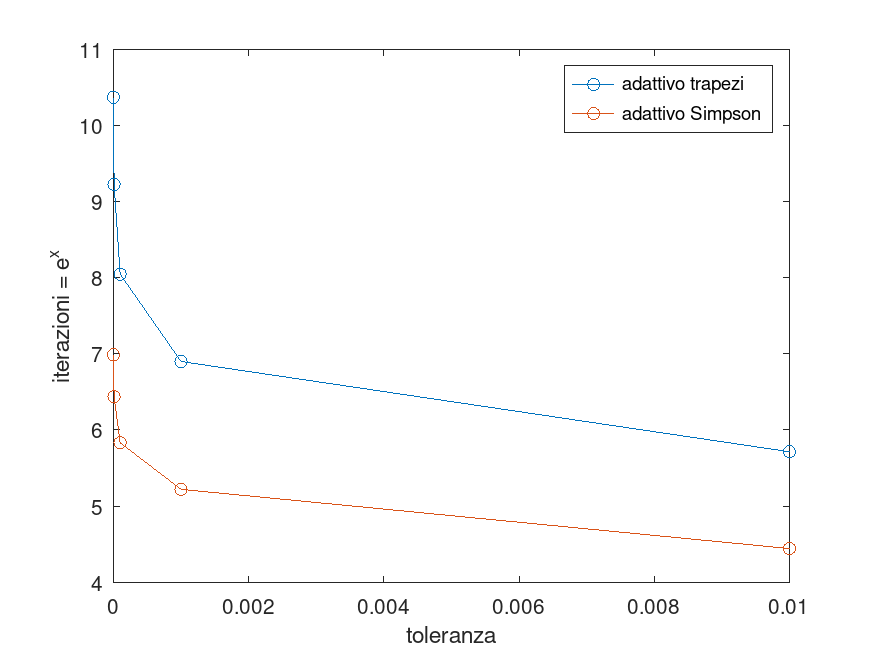
\includegraphics[width=16cm,height=10cm,keepaspectratio]{capitolo5/es30_figure.png}
    \caption{logaritmo di numero di valutazioni funzionali}
    \label{fig:es30}
\end{figure}
\FloatBarrier

\section{Codici ausiliari}

\subsection{Esercizio 6}
\lstinputlisting[caption=es6.m, label=cod:6]{./capitolo2/es6.m}

\subsection{Esercizio 7}
\lstinputlisting[caption=es7.m, label=cod:7]{./capitolo2/es7.m}

\subsection{Esercizio 15}
\lstinputlisting[caption=es15.m,label=cod:15]{./capitolo4/es15.m}

\subsection{Esercizio 16}
\lstinputlisting[caption=es16.m,label=cod:16]{./capitolo4/es16.m}

\subsection{Esercizio 18}
\lstinputlisting[caption=es18.m,label=cod:18]{./capitolo4/es18.m}

\subsection{Esercizio 19}
\lstinputlisting[caption=es19.m,label=cod:19]{./capitolo4/es19.m}

\subsection{Esercizio 20}
\lstinputlisting[caption=es20.m,label=cod:20]{./capitolo4/es20.m}

\subsection{Esercizio 21}
\lstinputlisting[caption=es21.m,label=cod:21]{./capitolo5/es21.m}

\subsection{Esercizio 22}
\lstinputlisting[caption=es22.m,label=cod:22]{./capitolo5/es22.m}

\subsection{Esercizio 23}
\lstinputlisting[caption=es23.m,label=cod:23]{./capitolo5/es23.m}

\subsection{Esercizio 24}
\lstinputlisting[caption=es24.m,label=cod:24]{./capitolo5/es24.m}

\subsection{Esercizio 25}
\lstinputlisting[caption=es25.m,label=cod:25]{./capitolo5/es25.m}

\newpage
\pagenumbering{roman}


\end{document}
